\documentclass[11pt]{article} % use larger type; default would be 10pt

% Common packages for mathematical articles
\usepackage{fullpage,amsmath,amsfonts,mathpazo,microtype,nicefrac,algorithm2e,graphicx}

% MSE Packages
\usepackage{caption}
\usepackage{physics}
\usepackage{xcolor}
\usepackage{listings}
\usepackage{parskip}

% MSE Make margins a bit smaller
\usepackage[margin=0.75in]{geometry}
\usepackage[font=footnotesize]{caption}

% MSE set graphics path
\graphicspath{{figs/}}

% Set-up for hypertext references
\usepackage{hyperref,color,textcomp}
\definecolor{webgreen}{rgb}{0,.35,0}
\definecolor{webbrown}{rgb}{.6,0,0}
\definecolor{RoyalBlue}{rgb}{0,0,0.9}
\hypersetup{
   colorlinks=true, linktocpage=true, pdfstartpage=3, pdfstartview=FitV,
   breaklinks=true, pdfpagemode=UseNone, pageanchor=true, pdfpagemode=UseOutlines,
   plainpages=false, bookmarksnumbered, bookmarksopen=true, bookmarksopenlevel=1,
   hypertexnames=true, pdfhighlight=/O,
   urlcolor=webbrown, linkcolor=RoyalBlue, citecolor=webgreen,
   pdfsubject={Harvard IACS AC 290 R},
   pdfkeywords={},
   pdfcreator={pdfLaTeX},
   pdfproducer={LaTeX with hyperref}
}
\hypersetup{pdftitle={AC290-RBC}}


% MSE Macros
\newcommand{\tty}[1]{\texttt{#1}}
\newcommand{\uu}{\vectorbold{u}}
\newcommand{\vv}{\vectorbold{u}}
\newcommand{\Laplace}{\Delta}

%***Start of Document***
\title{Numerical Simulation of Rayleigh-B\'enard Convection}
\author{Harvard IACS AC 290R - Group 1 \\
Michael S. Emanuel \\
Jonathan Guillotte-Blouin \\
Yue Sun \\
}
\date{14-March-2019} 

\begin{document}
\maketitle

\section{Problem Statement and Motivation}
AC 290R is a course on extreme computing with a focus on the application domain of fluid dynamics.
Fluid dynamics is one of the most mature areas of high performance computation.
Long before there were social networks, scientists and engineers have used 
the most powerful computers available to understand weather systems and aerodynamics.
For our project in this module, we carried out a large scale numerical simulation of 
Rayleigh-B\'enard Convection using the Drekar code running on Harvard's Odyssey supercomputing cluster.  
\href{https://en.wikipedia.org/wiki/Rayleigh%E2\%80%93B%C3%A9nard_convection}
{Rayleigh-B\'enard Convection} (RBC) is a classical problem in fluid dynamics.
It is the phyical phenomenon that arises any time a fluid in a gravitational field has a temperature gradient.
As anyone who lives in an old building can attest, hot air rises and cold air falls.  
This buoyancy effect of warm fluids expanding and becoming less dense is quite general.
When the temperature driven thermal forces are large enough compared to viscous forces,
the fluid will move with characteristic circular flows bringing hot fluid higher and cold fluid lower.
If the the thermal forces become large enough, a turbulent flow will emerge.

A number of scientifically important physical phenomena involve RBC.
Some of the more prominent ones include:
\begin{itemize}
\item\href{https://en.wikipedia.org/wiki/Stellar_evolution}{Stellar evolution}:
The gas at the center of a star is hotter than the gas at the outside, and a spherical RBC flow develops
\item\href{https://en.wikipedia.org/wiki/Plate_tectonics}{Plate tectonics}:
The hot center of the earth, with a layer of magma on top and a cool crust.  
Over geologic time scales, the earth's mantle behaves like a fluid, and plate tectonics is an instance of RBC.
\item{Weather systems}: Warm air rises in the earth's atmosphere and RBC drives weather processes. 
A concrete example is a \href{https://en.wikipedia.org/wiki/Mesoscale_convective_system}{mesoscale convective system}.
\end{itemize}

Our goals in this project are twofold.  
We would like to learn some basic precepts of fluid dynamics and gain a working knowledge of RBC.
We acknowledge however that fluid dynamics is far too large and complicated a field for us 
to gain a deep understanding in such a short time.
Our primary goal, as suggested by the course title \textbf{Extreme Computing}
is to learn state of the art techniques in scientific computing at a large scale.
We choose to work on a real problem, RBC, rather than a toy problem because
it is both more interesting and we will learn more.

The particular problem we simulated numerically is a two dimensional turbulent Rayleigh-B\'enard Convection.  
This is described mathematically with a set of three equations called the Boussinesq equations.
The \href{https://en.wikipedia.org/wiki/Boussinesq_approximation_(buoyancy)}{Boussinesq approximation} 
is based on a linearization of the buoyancy effect.
The buoyancy effect is approximated as 
$$ \rho(T_0 + \delta T) \approx \rho(T_0) - \frac{\partial \rho}{\partial T}\Bigr|_{T=T_0} \delta T$$
We define the coefficient of volume expansion as
\footnote{See here a discussion of  \href{https://en.wikipedia.org/wiki/Thermal_expansion}{thermal expansion} generally}
$$\alpha_V = -\frac{1}{\rho_0}\frac{\partial \rho}{\partial T}\Bigr|_{T=T_0}$$
The coefficient of volume expansion is a property of a fluid.
The second simplifying assumption made in the Boussinesq equations is that fluids are incompressible
(except for this linear sensitivity of their density to temperature).
The Navier-Stokes equations then simplify to the three Boussinesq equations:
\begin{align}
\frac{\partial \uu}{\partial t} + \grad \cdot (\uu \otimes \uu) &= \frac{1}{\rho_0} \grad P + \nu \grad^2 \uu + \alpha_V g T \hat{y} \\
\grad \cdot \uu &= 0 \\
\frac{\partial T}{\partial t} + \grad \cdot (uT) &= \kappa \grad^2 T
\end{align}

In these equations, $\rho_0$ is is the density at the reference temperature $T_0$.
$\nu$ is the fluid viscosity and $\kappa$ is the thermal diffusivity.

The presentation above includes the physical constants and is suitable for engineering.
For mathematics, it is often preferable to use nondimensional equations.
\footnote{See this article on the technique of \href{https://en.wikipedia.org/wiki/Nondimensionalization}{nomdimensionalization}.}
There are three choices that have been used for nondimensionalizing the Boussinesq equations.
We follow the classical approach and choose the following dimensionless parameters:
\begin{itemize}
\item{$\Delta T = T_{bot} - T_{top}$} the temperature difference; this is the temperature scale
\item{$H=y_{top} - y_{bot}$} the height of the channel; this is the length scale
\item{$\tau = \nicefrac{H^2}{\kappa}$} is the time scale; this choice is called ``thermal scaling''
\item{$U = \nicefrac{H}{\tau}$} is the velocity scale
\item{$\rho_0 U^2$} is the pressure scale
\end{itemize}

With this choice of dimensionless parameters, we have the non-dimensional Boussinesq equations:
\begin{align}
\frac{\partial \uu}{\partial t} + \grad \cdot (\uu \otimes \uu) &= \grad P + \textrm{Pr} \grad^2 \uu + \textrm{RaPr}T \hat{y} \\
\grad \cdot \uu &= 0 \\
\frac{\partial T}{\partial t} + \grad \cdot (uT) &=  \grad^2 T
\end{align}

There are two dimensionless ratios appearing:
\begin{itemize}
\item{Pr} is the \href{https://en.wikipedia.org/wiki/Prandtl_number}{Prandtl number}, $\textrm{Pr} = \nicefrac{\nu}{\kappa}$.  
This is the ratio of the thermal viscosity to the thermal diffusivity and is a property of the fluid.
\item{Ra} is the famous \href{https://en.wikipedia.org/wiki/Rayleigh_number}{Rayleigh number}.  It is defined by
$$\textrm{Ra} = \frac{\alpha_V \Laplace T g H^3}{\nu \kappa}$$
The Rayleigh number describes the ratio of temperature driven forces to viscous forces.
For this reason, a very low Rayleigh number leads to no convective flow; 
an intermediate Rayleigh number leads to a somewhat regular flow;
and a high Rayleigh number leads to a turbulent flow.
\end{itemize}

\section{Description of Code}
Drekar is a large scale computational fluid dynamics (CFD) code.
The name Drekar comes from the norse word describing a 
\href{https://en.wikipedia.org/wiki/Longship}{Viking Longship}.
It is under active development at \href{https://www.sandia.gov/}{Sandia National Laboratories}
and was recently made partially open source; details can be found at the US Department of Energy
Office of Scientific and Technical Information at \href{https://www.osti.gov/biblio/1364765}{OSTI.gov}.
Because some parts of this code are sensitive, e.g. they could be used for simulations of nuclear weapons,
these parts are not being released to the public.
Sensitive components will remain restricted to employees and affiliates of Sandia.


Drekar solves the partial differential equations (PDEs) of fluids using the Finite Element Method.
In addition to simulating traditional fluid dynamics problems, Drekar also has the capability to handle
electromagnetic forces.  This is important when modeling plasma physics and stars for example.
Drekar is able to accurately simulate different kinds of physical systems including incompressible fluids,
low-mach compressible fluids, and compressible / incompressible magnetohydrodynamics.
It can also handle multi-species plasmas interacting with a magnetic field;
this is used to simulate \href{https://en.wikipedia.org/wiki/Tokamak}{Tokamak} reactors.
Researchers at Sandia are collaborating with the team building the \href{https://en.wikipedia.org/wiki/ITER}{ITER}
in Southern france, which will be the world's largest megnetic confinement plasma physics experiment when
it is constructed.

The heart of Drekar is a massively parallel implementation of the 
\href{https://en.wikipedia.org/wiki/Finite_element_method}{Finite Element Method}.
The Finite Element Method is a numerical method for solving partial differential equations.
We will discuss it further in the next section.
Drekar is a modern software project written in C++ and making extensive use of classes and templates.  
This allows it to be flexible and to run efficiently on heterogeneous hardware.

Drekar implements parallelization at multiple levels.
At the top level, it uses 
\href{https://en.wikipedia.org/wiki/Message_Passing_Interface}{Message Passing Interface} (MPI)
to distribute computations across multiple computing nodes that are connected on
the same high performance network.
Back end modules of Drekar also permit parallelization at the level of C++ threads;
\href{https://en.wikipedia.org/wiki/OpenMP}{OpenMP} (multiple cores on one host); 
and GPUs with \href{https://en.wikipedia.org/wiki/CUDA}{CUDA}.

Drekar has basic components that handle primitive linear algebra tasks such as 
distributing a matrix or a vector across multiple compute nodes.
Building up in complexity, it knows how to add vectors,
perform vector dot products and matrix / vector products.
It can solve linear equations exactly or approximately using Krylov methods,
and similarly for eigenvalue problems.
And it can solve nonlinear equations using iterative methods
(typically refinements of Newton's method).

These building blocks enable Drekar to simulate a wide variety of PDEs
using the finite element method, and to perform these scales efficiently at scale.
Drekar handles continuous, discontinuous and stabilized finite elements.
The flexibility and wide range of the C++ classes in Drekar allow it to simulate
mixed-integration finite element bases including nodal, edge, face, and volume elements.
This allows a wide range of problems to be described.
The breadth of elements are particularly useful when enforcing complex boundary conditions.
Drekar also has the flexibility of simulating multiple physics regimes, called blocks, in one system.

Drekar includes algorithms for time integrating differential equations that are 
fully explicit, fully implicit, and mixed implicit / explicit (IMEX).  
Some degree of implicit solution is often required for real world problems
when there is a wide range of time scales.  If the fastest time scale
is too many orders of magnitude shorter than the longest one,
an explicit solver will either take time steps too large to capture the physics,
or take too long to run.  
Implicit and IMEX solvers permit the simulation to implicitly solve for physical
effects that are on too short a time scale to solve explicitly.

Drekar has strong tools for automatic differentiation.
These are necessary because many methods used in Drekar require
taking derivatives of functions, e.g. solving nonlinear equations with a variant of Newton's method.  
Some other software libraries required users to supply hand coded derivatives, 
which can be time consuming and error prone;
or to use numerical derivatives, which can be slow.
Automatic differentiation allows the best of both worlds.

Drekar is built as a part of a collection of packages called
\href{https://trilinos.github.io/}{Trilinos}.
Trilinos arose out of an effort at Sandia to avoid duplication of effort across
different research groups and allow each group to focus on the frontier
of discovery in their area without reinventing the wheel.
Some packages in Trilinos relevant to Drekar include:
\begin{itemize}
\item{\textbf{Linear solvers}}: \textit{Amesos} (direct) and \textit{Aztec00}, \textit{Belos} (indirect)
\item{\textbf{Preconditioners}}: \textit{lfpack} (algebraic), \textit{ML} (multilevel), \textit{Meros} (block)
\item{\textbf{Eigenvalue solvers}}: \textit{Anasazi}
\item{\textbf{Nonlinear solvers}}: \textit{NOX}
\item{\textbf{Time Integrators}}: \textit{Rhythmos, Tempus}
\item{\textbf{Automatic Differentiation}}: \textit{Sacado}
\end{itemize}
Consider for a moment how many of the basic building blocks used by Drekar
are provided by the packages listed above.
By building on this existing work, the developers of Drekar were able 
to concentrate their efforts on the distinctive aspects of the problem,
namely solving PDEs with the Finite Element Method.
Having seen a number of software packages over the year, 
our first impression of Drekar is that it is a very sophisticated 
and impressive piece of software engineering.

\subsection{The Software Behind The Simulation}

We will spare you with the details of building Drekar and Trilinos, as we essentially followed word for word the instructions presented in 
\href{https://github.com/dsondak/DrekarBase/blob/master/README.md}{the repo's README}.

Once that was done, we experimented with toy examples --- for instance, 64x64 grids on just a single Odyssey core --- 
to see how Drekar behaved, and how to gather its \textit{.exo} output. To visualize the output, we used ParaView, 
which is another software tool built at Sandia labs; in our case, we could download the \textit{.exo} file to our local machine, 
import it to the ParaView GUI, and then fiddle with the vast array of visualization features. 
That strategy could not scale with realistic simulation output, which can be on the terabyte scale, 
but it was good enough to get used to the tools and to prototype.

As for running Drekar, three input files were particularly important: \textit{case1.sh}, \textit{case1.pam}, and \textit{case1.xml}. 
Because the simulation is compute-heavy and takes a long time to run, it was not reasonable to run it on 
either login nodes, or via an interactive session. 
Therefore, we wrote \textit{case1.sh}, which defines the various SLURM flags, and parameters for the simulation
to be run as a batch job on Odyssey using \textit{sbatch case1.sh}. 
In the end, this batch job runs the Drekar executable with \textit{case1.xml} as input. 
The XML file describes pretty much all the information about the desired environment in order for Drekar to run properly. 
Indeed, Drekar by itself (including Trilinos) is a gigantic optimized toolkit, but it is not compiled with a series of specific actions to do. 
Fortunately, the behaviour we want to emulate can be written in an XML or YAML file, which is then dynamically parsed by Drekar afterwards. 
We can set crucial information like boundary counditions, time steps, solvers, and so on, without having to implement any of it (or very little). 
The XML file contains two other important pieces of information: the path to the \textit{.exo} output, 
as well as the pamgen input for the grid specification. 
The exodus file is yet another creation of Sandia labs, which aims at storing and accessing finite element analyses.\cite{exo} 
It is important to note that if Drekar is running on $n$ cores in parallel, $n$ exodus files are created 
and updated over the course of the simulation. 
Once the simulation is over, it might be useful to combine all these partitioned files into a single exodus files: 
to do that, we use the epu CLI application. However, that last step is not necessary if we only want to visualize
 the analyses using ParaView, as it can handle both having the partitioned files, or the combined exodus output.  
This brings us to the last file: \textit{case1.pam}.  
Pamgen is a technology which enables us to easily define the mesh used during our finite element analysis.\cite{pam} 
We could have used other tools to generate such mesh, but Pamgen is a popular approach which we were presented in the context of this class.


\section{Overview of Numerical Methods Used}
The main numerical methods used in Drekar are the Finite Element Method (FEM)
and nonlinear equation solvers.
The Finite Element Method discretizes a partial differential equation in space.
The spatial discretization is carried out by dividing the space into a collection of
subdomains called a \textit{mesh}.  
For example, on the RBC problem, we divide the $x$ direction into 2048 evenly spaced
points and the $y$ direction into 1024 points with Chebyshev spacing.

We then try to solve the PDE on a finite dimensional space of functions.
We replace the infinite dimensional space of functions on the domain with a finite
dimensional function space by introducing a \textbf{basis} of functions defined on each element.
The choice of basis is important.  
Different bases give rise to different methods, and some work better on different problems than others.
Drekar has the capability to use a number of different bases for the FEM.
As a concrete example of this technique, on our homework assignment we solved the Poisson
equation with the FEM by using the basis piecewise linear functions 
connecting two adjacent nodes.  
This was a direct solve to a steady state rather than a time integration,
but it illustrates the mechanics of the FEM.

Once a basis has been chosen, the state of the system at a moment in time
can be described by assigning weights to each basis vector.  
This also allows us to describe the evolution of the system over one discrete
time step by applying the differential equation in this basis.
If we use an explicit time step as we did on the 1D Poisson problem
example, we will end up with a linear equation to solve at each time step.

For a more complex system, we will often need to solve a nonlinear equation
to advance the system from one time step to the next.
Implicit solvers (including an IMEX solver) will often require the solution of a nonlinear equation.
To make this a bit more concrete, consider two different ways discretize one
step of the 1D Poisson equation in time:
\begin{align}
\frac{u^{n+1}_{j} - u^{n}_{j}}{k} &= \frac{u^{n}_{j+1} - 2u^{n}_{j} + u^{n}_{j+1} }{h^2} \\
\frac{u^{n+1}_{j} - u^{n}_{j}}{k} &= \frac{u^{n+1}_{j+1} - 2u^{n+1}_{j} + u^{n+1}_{j+1} }{h^2}
\end{align}

The superscript $n$ or $n+1$ indicates the time step.  
The subscript $j$ indicates the spatial grid entry.
While these two equations look superficially similar, they describe very different algorithms, 
which would become clear if you tried to program them on a computer.
The first equation is \textbf{explicit}.  The right hand side is known at time step $n$.
It allows us to solve for the new value $u^{n+1}_{j}$ explicitly in terms of known quantities at time step $n$.
This makes it easy to program and intuitive.
The next equation though is \textbf{implicit}.  
It defines a relationship between the $u_{n+1}$ but the right hand side is not known at time step $n$.
Instead of evaluating $u^{n}_{j}$ directly, a system of linear equations must be solved.
In more complicated differential equations, using implicit time steps leads to nonlinear equations.

The basic technique used to solve nonlinear equations is usually some variant of Newton's Method.
In Newton's method, we attempt to solve the nonlinear equation $F(X) = 0$ iteratively as follows.
We make an initial guess $X_0$ and evaluate the residual $r = F(X_0)$ and the Jacobian (derivative) $J$.
We then make a new guess using the approximation that $F$ is locally linear,
i.e. we apply a shift $\Delta X$ such that $J \Delta X = -r$.
This simple method works amazing well, but it can fail to converge if a function
has too large a second derivative or if a bad initial guess is made.

Nonlinear solvers are a mature field in applied mathematics with their own rich tradition.
We learned during the guest lecture of a few of the advanced techniques 
used in Trilinos (NOX) for solving nonlinear equations:
\begin{itemize}
\item{\textbf(line search)} rather than applying the full $\Delta x$ implied by Newton's method,
perform a line search in that direction; often the step size chosen will be smaller
\item{\textbf{trust region}} by comparing the predicted and actual function values,
maintain an estimate of how large a region the derivative approximation is valid
for.  When taking a step, limit it to this trust region.
\item{\textbf{second derivative methods}} build up an estimate of the second derivative as well
as the first derivative and use it for a sharper estimate of the step to take
\item{\textbf{homotopy methods}} identify a parameter in the equation that governs its behavior.
It should allow for a simpler solution when the value changes 
(e.g. solving RBC is easier when the Rayleigh number is lower).
Solve the system at an easy setting, then use that solution as the initial guess
 for a new solution at a higher setting.  Gradually iterate to the solution at
 the desired parameter value.
\end{itemize}

A third important idea in the numerical solution of differential equations is adaptive time steps.
An adaptive solver formulates an estimate of the error at a time step.  
If the error exceeds a tolerance (which is an input parameter) the step is rejected and 
a new attempt is made with a smaller time step.
Adaptive time steps can be beneficial on problems where there is more ``action'' in the
system at some times than others.  
The classic example of this phenomenon in introductory graduate courses on this
topic is the Brusselator system from chemical kinetics.

\section{Parameters of the Simulation}
All parameters to the simulation are input with a configuration file.
This can be passed in either XML format (the old technique) or YML (the new technique).
We were provided with a template XML file which we then modified to incorporate the 
specific parameter settings.
We made two simulation runs, \textbf{case 1} (on 512 cores for about a day)
and \textbf{case 2} (on 1024 for about 5 days).  
There was a slight change in parameter values explained below.

We generated a mesh using a program called Pamgen.  Here are the key parameters for the mesh (spatial layout):
\begin{itemize}
\item{length} $L=2$  with $N_x = 2048 + 1$ uniformly spaced mesh points
\item{height} $H=1$ with $N_y = 1024 + 1$ Chebyshev spaced mesh points
\item{$\Gamma = \nicefrac{L}{H} = 2$}
\item{x} ranges from 0 to 2
\item{y} ranges from 0 to 1
\end{itemize}

Here are descriptions of the key physical parameters for the simulation
\begin{itemize}
\item{\textbf{density}} $\rho_0 = 1.0$
\item{\textbf{viscosity}} $\nu = 0.01$
\item{\textbf{volume expansion coefficient}} $\alpha_V = 10^6$
\item{\textbf{gravity}} $g = 1.0$
\item{\textbf{heat capacity}} $C_p = 1.0$
\item{\textbf{thermal conductivity}} $k = 0.01$
\item{\textbf{thermal diffusivity}} $\kappa = \nicefrac{k}{\rho C_p} = 0.01$
\item{\textbf{temperature change}} $\Delta T = 1.0$ 
\item{\textbf{height}} $H = 1.0$
\item{\textbf{time of simulation}} we attempted to simulate from time $t=0$ to $t=5$.
\end{itemize}

Using these parameters, we can compute the implied dimensionless constants:
\begin{align}
\textrm{Pr} &= \frac{\nu}{\kappa} = \frac{0.01}{0.01} = 1.0 \\
\textrm{Ra} &= \frac{\alpha_V \Delta T g H^3}{\nu \kappa} = \frac{10^{6} \cdot 1.0 \cdot 1^3}{0.01 \cdot 0.01} = \frac{10^{6}}{10^{-4}} = 10^{10}
\end{align}
We comment in passing that in order to achieve the required Rayleigh constant of $10^{10}$, 
we solved for the required volume expansion coefficient $\alpha_V$ given the other parameter settings.

In addition to the phyiscal constants, some additional parameters were passed to Drekar 
specifying the boundary conditions and how the physics should be modeled.
Important settings of this type included:
\begin{itemize}
\item{\textbf{Initial conditions}} $U_x = 0$, $U_y = 0$, $P = 0$.  The velocity and pressure started uniformly zero.\\
On our initial run with 512 cores (case 1), the temperature starts with a trigonometric function from 0 to 1
which is the analytical solution at steady state on an infinite plane first worked out by Rayleigh. \\
We observed that the solver had a difficult time ramping up under these conditions 
due to the highly turbulent flow at $\textrm{Ra} = 10^{10}$.  
For this reason we changed the initial conditions on our second run, case 2. 
\item{\textbf{No slip boundary condition}} $U_x = 0$, $U_y = 0$ 
on the top (surface\_4) and bottom (surface\_2).
\item{\textbf{Applied temperature gradient}} $T=0$ at the top, $T=1$ at the bottom; therefore $\Delta T = 1$.
This is true for all time $t$ in case 1.  
In case 2, we set the temperature at the bottom plate to be 
$T(t) = 1 - e^{-t / \tau}$ where the time scale $\tau$ for ramping up the temperature was $\tau = 0.2$.
This is an example of the technique of \textit{parameter continuation}.
\item{Finite element basis for PDEs} The continuity, momentum and energy equations all share the same
finite element settings.  The basis is HGrad of order 1 with integration order 2.  Stabilization is on.
The basis HGrad consists of piecewise polynomial elements.  
When the order is 1, this is the familiar piecewise linear function in 1D.
For our case of a 2D planar domain, the elements are still piecewise linear, 
but on recetangular tiles rather than line segments.
\item{Stress tensor} is modeled as Newtonian.
\item{Source momentum} is modeled with the Boussinesq approximation; 
using a reference density of 1.0 and a reference temperature of 0.5, the mean for the simulation.
\end{itemize}

\section{Results}
We made two simulation runs:
\begin{itemize}
\item{\textbf{case 1}} Our first run was intended to run on 1024 CPU cores but only ran on 512 cores due to a hardware fault.
We terminated it and restarted it when the problem was diagnosed and corrected.  We ended up with 22.7 GB of output
encompassing about 0.22 of simulation time of 5.0 desired.
\item{\textbf{case 2}} We ran a second batch, starting from scratch rather than re-starting case 1.
This was run on the full 1024 cores.  However, the run terminated early when it crashed due to running out of memory.
Diagnostics reveal that it also steadily slowed down during the simulation, ending up with only 0.77 time units.
The output files appear to have become corrupted as a result of the crash and may be unusable.
Based on the observed pattern of steadily deteriorating performance followed by an out of memory error,
we suspect there may be a memory leak in Drekar that only manifested on our compilation when we ran
the large job for an extended time.
\end{itemize}

We must admit to a measure of disappointment that our largest simulation run did not successfully complete.
However if you try something and know the result ahead of time, 
what you're doing might be instructive but probably isn't science!

On a more fun note, here are some visuals from the successful albeit short case 1 run.
We present some still images here in the report, but the pi\`ece de r\'esistance 
is the \href{https://youtu.be/1DIGnRgUhe4}{movie}.

\newpage
% temperature image
\subsection{Temperature Field}
Temperature field presents direct visualizations of the temperature distribution in the flow, and illustrates the motion of the flow. Figure 1 is the temperature field at $t=0.189$, where cold colors represent the low and the warm colors represent the high temperature. It also shows some nice swirls and eddies in the flow. As time elapsed, high temperature diffuses in the flow, while the bottom still preserves higher temperature, which is in accordance to the initial temperature condition. For better visualization, we cap the maximum value on the colorbar 
at $0.25$, and use both \texttt{pcolormesh} and \texttt{contourf} approach.
\begin{figure}[h!]
\centering
\hspace*{-0.25in}
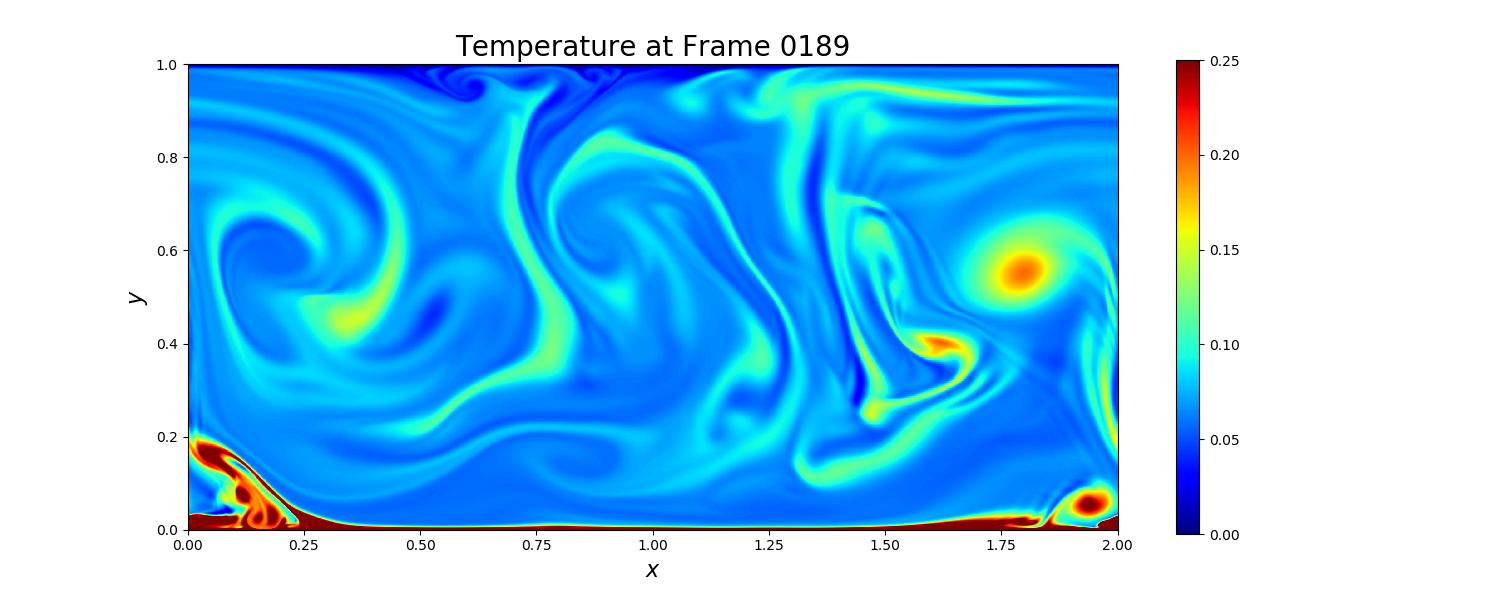
\includegraphics[width=1.2\textwidth]{temperature.png}
\caption{Mesh plot of the temperature field at $t=0.189$.}
\hspace*{-0.25in}
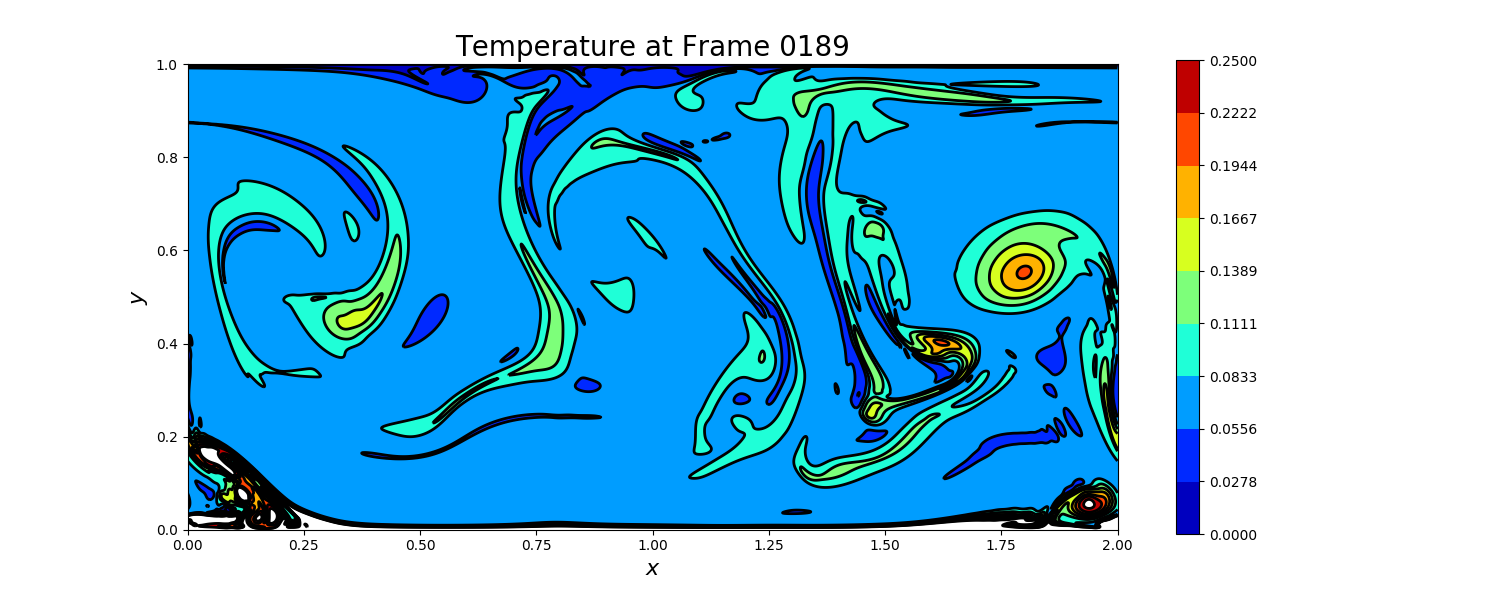
\includegraphics[width=1.2\textwidth]{temperature_contour.png}
\caption{Contour plot of the temperature field at $t=0.189$.}
\end{figure}
\newpage

% Nusselt number
\subsection{Nusselt Number}
With the visualizations of the temperature field at hand, it is nature to study the quantitative behavior of the heat transport. The Nusselt Number is the primary dignostic quantity used to measure vertical heat transport.  It is a dimensionless quantity that indicates the ratio of total heat transport to heat transport from conduction alone.  A value of 1.0 indicates heat transport due only to conduction.
The range of values below between 3 and 4 indicates a flow with quite
a lot of heat transport due to hotter fluid rising.  
This is as expected in a flow with such a high Rayleigh number.

\begin{figure}[h!]
\centering
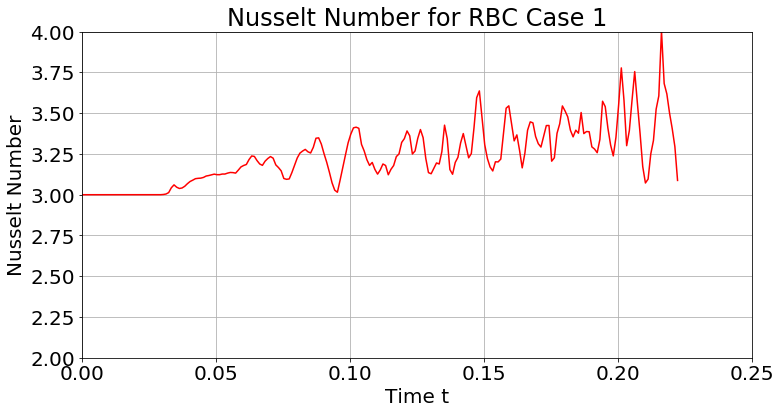
\includegraphics[width=0.5\textwidth]{nusselt.png}
\caption{Nusselt number from $t=0$ to $t=0.224$.}
\end{figure}

% pressure image
\subsection{Pressure Field}
\textbf{Some words on the pressure field.}
\begin{figure}[h!]
\centering
\hspace*{-0.25in}
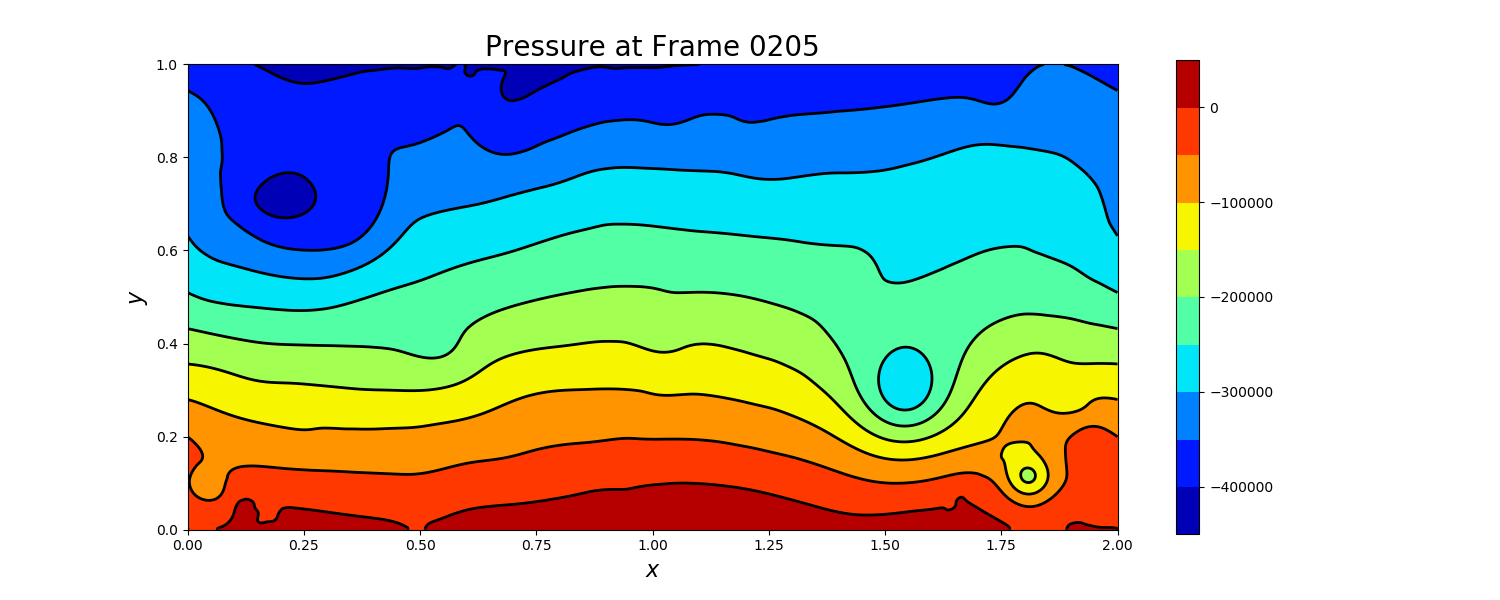
\includegraphics[width=1.2\textwidth]{pressure.png}
\caption{Contour plot of the pressure field at $t=0.205$.}
\end{figure}
\newpage

% velocity x image
% velocity y image
\subsection{Velocity Field}
Since the velocity field is a vector field, we visualize the $x$ and $y$ components independently. 

\textbf{Some explanation on the color bar.}
\begin{figure}[h!]
\centering
\hspace*{-0.25in}
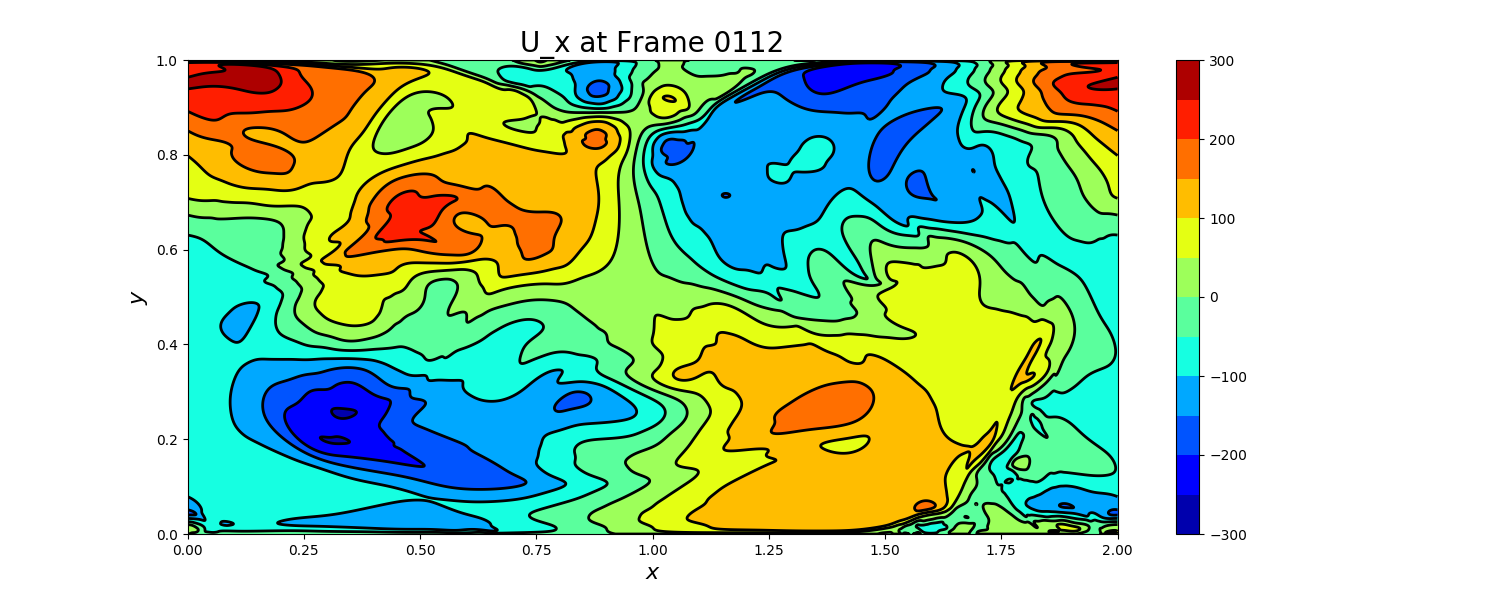
\includegraphics[width=1.2\textwidth]{velocity_x.png}
\caption{Contour plot of the velocity field in $x$ component at $t=0.112$.}
\hspace*{-0.25in}
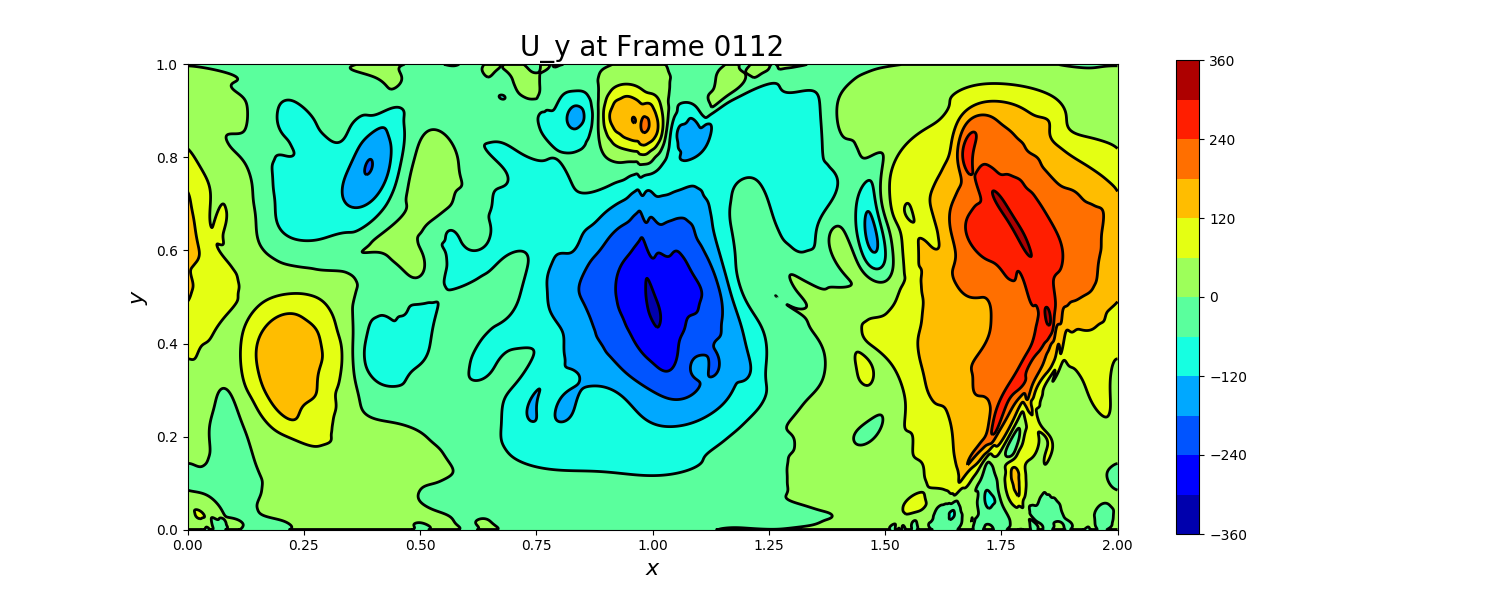
\includegraphics[width=1.2\textwidth]{velocity_y.png}
\caption{Contour plot of the velocity field in $y$ component at $t=0.112$.}
\end{figure}
\newpage

% streamline image
\subsection{Streamline Field}
Another visualization to understand the velocity field is to plot the streamlines, which show the motion of the flow. We present two ways to plot the streamlines: First we overlay the velocity magnitude field with the streamline; second we color the streamlines with the temperature, and change its width to represent the velocity magnitude, which confers information about the flow temperature and velocity.

\begin{figure}[h!]
\centering
\hspace*{-0.25in}
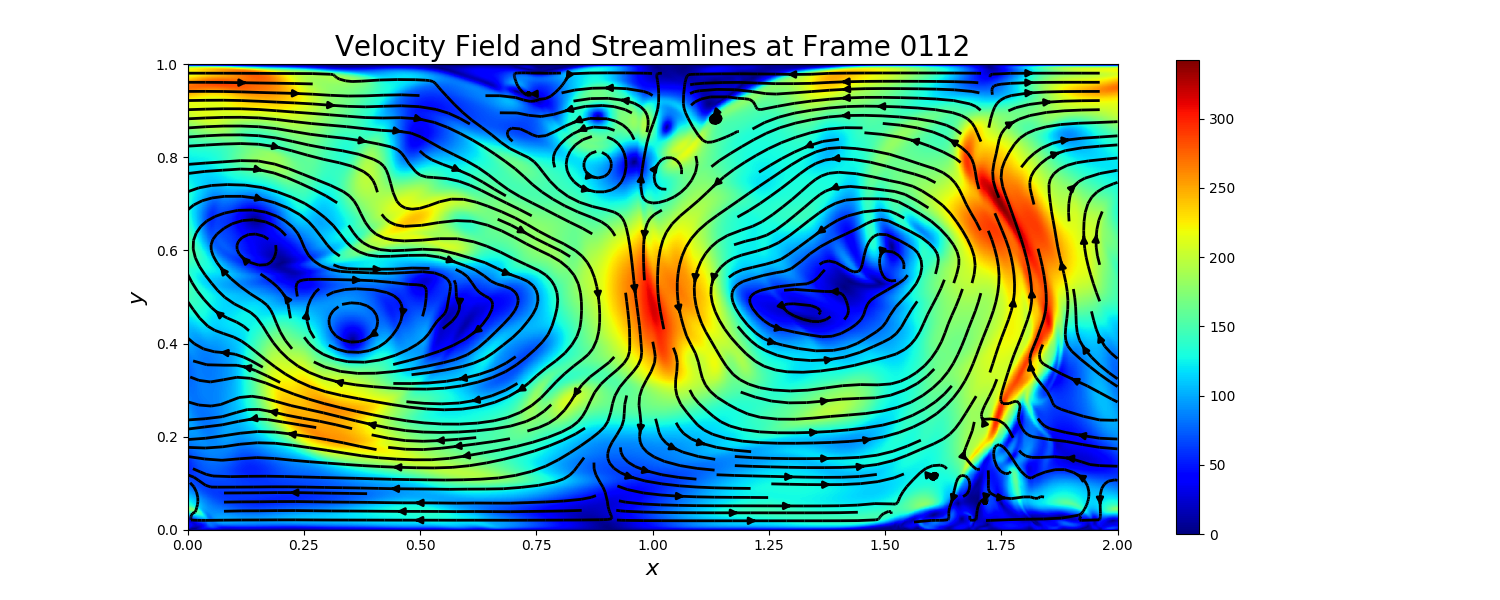
\includegraphics[width=1.2\textwidth]{streamline_regular.png}
\caption{Contour plot of the velocity field in $x$ component at $t=0.112$.}
\hspace*{-0.25in}
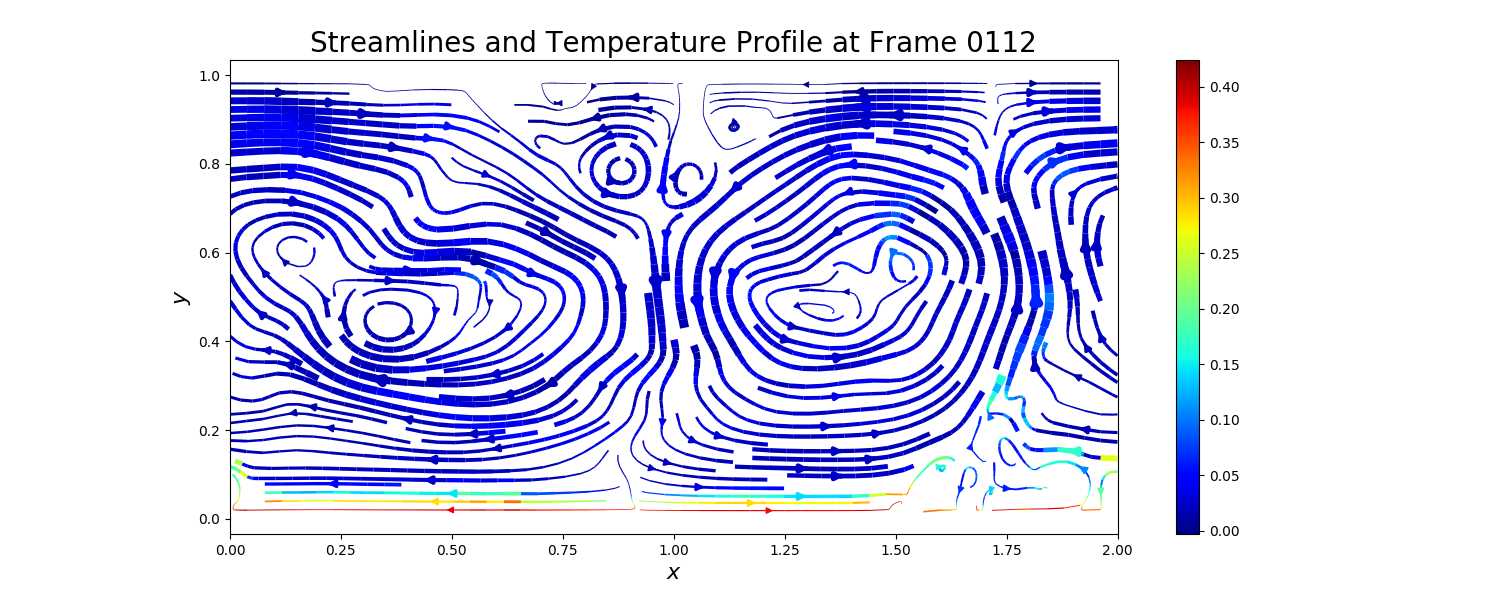
\includegraphics[width=1.2\textwidth]{streamline.png}
\caption{Contour plot of the velocity field in $y$ component at $t=0.112$.}
\end{figure}
\newpage

\subsection{Schlieren Flow Visualization}
Schlieren flow visualization enhances the features and the structures of eddies and swirls of the flow, which is complementary to the previous fields visualizations. Typically Schlieren images are rendered in grey-scale for comparisons with experimental data.  
\begin{figure}[h!]
\centering
% \hspace*{-0.25in}
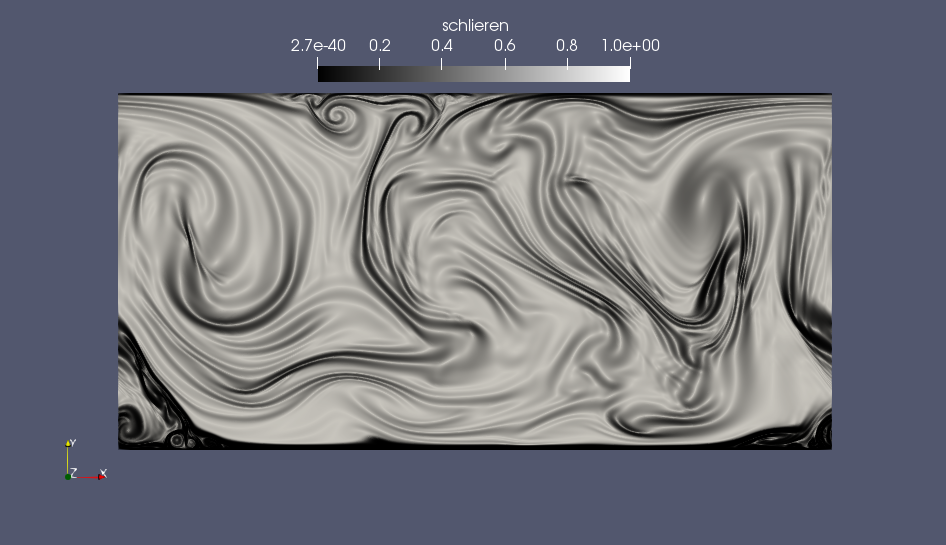
\includegraphics[width=0.7\textwidth]{schlierin_grey.png}
\caption{Contour plot of the velocity field in $x$ component at $t=0.112$.}
\end{figure}


\newpage
\section{Conclusions and Future Work}
Extreme scale computing is a rich field that is at the leading edge of scientific discovery.
Our first brief foray was sufficient to give us a sense of the kinds of problems that can
be solved with these techniques.  
It is also humbling to learn how much we don't know.  
Becoming proficient in this field would take months and expertise would require years.

We've seen the power of the Finite Element Method and the tremendous capabilities of 
a research code like Drekar.  
We've also felt the pain of trying to compile Drekar from source and configure a job.
There are some software projects you can build by typing\\
\tty{git clone my\_program}\\
\tty{ make my\_program} \\
Drekar is not one of them!

One obvious piece of future work is to get to the bottom of the performance slowdown 
and out of memory error that brought simulation case 2 down.
Once the problem is repaired, we would like the opportunity to run the job to completion.
We understand that may not be possible due to constraints on computing resources
but would like to try. 

For visualization it would be cool to have several trace particles, and plot their trajectories along the flow. In addition, painterly rendering in computer graphics can be used to render each frame, which would truly create a painterly like water flow, like Van Gogh or Hokusai.

%% bibliography

\begin{thebibliography}{9}
\bibitem{exo} 
Schoof, L. A., \& Yarberry, V. R. (1994). EXODUS II: a finite element data model (No. SAND-92-2137). Sandia National Labs., Albuquerque, NM (United States).

\bibitem{pam}
DRAKE, R., FOUCAR, J., HENSINGER, D., WONG, M., BUDGE, K., \& GARDINER, T. (2008). Pamgen (No. PAMGEN; 002393WKSTN00). Sandia National Laboratories.

\bibitem{colorpalette}
Paintings Color Palettes: \url{https://designshack.net/articles/inspiration/10http:/designshack.net/articles/inspiration/10-free-color-palettes-from-10-famous-paintings/}

\end{thebibliography}

\end{document}
